% !TEX root = ../fys_cursus.tex



\chapter{Eendimensionale bewegingen}

Beweging beschrijven is niet zo simpel als het in eerste instantie lijkt. Zo is bijvoorbeeld de beweging van een wolk eerder complex. Wat reken je al dan niet tot de wolk? Ook de bewegingen van de afzonderlijke moleculen in kaart brengen is een onmogelijke opgave omdat het aantal moleculen eerder groot is. Om toch vooruitgang te kunnen boeken, beginnen we met voorwerpen die we als een punt kunnen voorstellen. We maken dan abstractie van de ruimtelijke vorm van het object dat we beschrijven en doen alsof we het kunnen reduceren tot \'e\'en enkele plaats in de ruimte. Zo zouden we het vliegen van een vlieg doorheen de kamer kunnen bekijken als een stipje. Het bewegen van de vleugels of de ori\"entatie van de kop van de vlieg laten we dan buiten beschouwing. Ook deze beschrijving kunnen we inperken; we gaan in eerste instantie enkel bewegingen beschrijven die voor te stellen zijn op een rechte lijn. Dit noemen we eendimensionale bewegingen. Als we de beschrijving hiervan eenmaal kennen, kunnen we later dit met behulp van vectoren gemakkelijk uitbreiden naar een beschrijving van bewegingen in twee- of drie dimensies.

Om het ons gemakkelijk te maken, zullen we in dit hoofdstuk enkel werken met de getalcomponenten van de vectoren. Dat gaat omdat we steeds in \'e\'en dimensie werken en de eenheidsvector dan steeds gelijk blijft. Als we $v_x$ kennen, vinden we direct de vectorcomponent volgens de $x$-as met $\vec{v}_x=v_x\cdot\vec{e}_x$. Bovendien kunnen we de index $x$ ook weglaten. We weten dat het steeds over de $x$-as gaat.

\section{Enkele begrippen}
\subsection{Positie en plaatsfunctie}

Het beschrijven van de beweging van een puntmassa kunnen we doen door de positie in de ruimte te geven in functie van de tijd. We kunnen m.a.w. een functie gebruiken die de plaats in functie van de tijd geeft. We noemen deze functie de \emph{plaatsfunctie} $x(t)$. $x$ staat voor de positie op een co\"ordinaatas\footnote{Een co\"ordinaatas is een as van een cartesiaans assenstelsel, met een oorsprong en een ori\"entatie.} en $t$ is de variabele die symbool staat voor de tijd\footnote{In de fysica gebruiken we de wiskunde als `taal' om de wetmatigheden van de natuur in uit te drukken. Wiskundige variabelen en objecten zoals functies krijgen nu een fysische betekenis. $x(t)$ is dus niets anders dan een functie $f(x)$ of $y(x)$ zoals je die in wiskunde kent. Alleen nemen wij nu niet voor de onafhankelijke variabele het symbool $x$ maar het symbool $t$ omdat deze symbool moet staan voor de tijd. En voor het symbool $f$ gebruiken wij nu het symbool $x$ omdat de beeldwaarden van de functie nu als betekenis een positie op een co\"ordinaatas hebben.}. Een notatie voor een bepaalde posities \footnote{Natuurlijk kan de index 1 ook vervangen worden door andere indices. Voorbeelden zijn $x_0=x(t_0)$ en $x_2=x(t_2)$.} op de co\"ordinaatas op een bepaald tijdstip $t_1$, is:
\begin{eqnarray*}
x_1=x(t_1)
\end{eqnarray*}
Zo zie je in figuur (\ref{grafplaatsfunctie}) een auto op verschillende tijdstippen $t_0,t_1, t_2,\ldots$ weer\-ge\-ge\-ven op verschillende posities. Je ziet ook een grafiek van de bijbehorende plaatsfunctie.

\begin{figure}[h]
\hfill
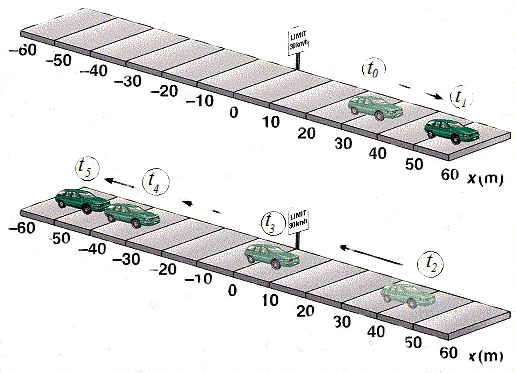
\includegraphics[width=0.45\textwidth]{Serway2p1(1)}
\hfill
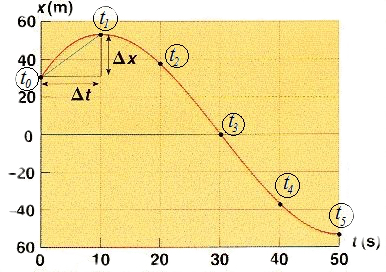
\includegraphics[width=0.45\textwidth]{Serway2p1(2)}
\hfill
\caption{Verschillende posities en de grafiek van de plaatsfunctie}
\label{grafplaatsfunctie}
\end{figure}

Het verschil tussen twee co\"ordinaten noemen we de \emph{verplaatsing}:
\[
\Delta x = x_2-x_1
\]
Zo is de verplaatsing van de auto in de figuur tussen de tijdstippen $t_0$ en $t_1$ gelijk aan $\Delta x = x_1-x_0=50\rm\,m-30\rm\,m=20\rm\,m$ en is de verplaatsing tussen de tijdstippen $t_2$ en $t_4$ gelijk aan $\Delta x=x_4-x_2=-40\rm\,m-40\rm\,m=-80\rm\,m$. Deze laatste verplaatsing is negatief, wat aangeeft dat de auto netto naar achteren is bewogen -- tegengesteld aan de zin van de gekozen as.
\newline
Let op, de verplaatsing hoeft niet noodzakelijk gelijk te zijn aan de \emph{afgelegde weg} tussen de twee bijbehorende tijdstippen. Als je op caf\'e na naar het toilet te zijn geweest terug op je oorspronkelijke plaats op het terras gaat zitten, is je (netto) verplaatsing nul maar heb je wel degelijk afstand afgelegd.

\subsection{Gemiddelde snelheid}

De gemiddelde snelheid $\overline{v}$ \footnote{Als symbool voor de gemiddelde snelheid wordt ook $<v>$ gebruikt.} van een voorwerp tussen twee tijdstippen defini\"eren we als de verplaatsing over het benodigde tijdsinterval.
\begin{eqnarray*}
\overline{v}=\frac{\Delta x}{\Delta t}=\frac{x_2-x_1}{t_2-t_1}
\end{eqnarray*}
De eenheid van snelheid is bijgevolg meter per seconde $[v]=\rm\,m/s$. Als voorbeeld is de gemiddelde snelheid van de auto in figuur (\ref{grafplaatsfunctie}) tussen de tijdstippen $t_1$ en $t_2$ gelijk aan $\overline{v}=\frac{x_2-x_1}{t_2-t_1}=\frac{40\rm\,m-50\rm\,m}{20\rm\,s-10\rm\,s}=-1\rm\,m/s$. Dat de snelheid negatief is, betekent natuurlijk dat de auto achteruit rijdt.

\subsection{Gemiddelde versnelling}

Zoals we bij snelheid kijken hoe de positie verandert gedurende de tijd, kunnen we ons ook afvragen hoe de snelheid verandert gedurende de tijd. Dit idee ken je al, we noemen het versnellen of vertragen.

De gemiddelde versnelling tussen twee tijdstippen defini\"eren we als de verandering van de snelheid in het bijbehorende tijdsinterval.
\begin{eqnarray*}
\overline{a}=\frac{\Delta v}{\Delta t}=\frac{v_2-v_1}{t_2-t_1}
\end{eqnarray*}
De eenheid van versnelling is bijgevolg meter per seconde, per seconde -- wat meter per seconde in het kwadraat geeft $[a]=\rm\,m/s^2$.

\subsection{Ogenblikkelijke snelheid}

Zoals we een voorwerp op een bepaald tijdstip een positie toekennen, willen we het voorwerp ook een snelheid op een bepaald tijdstip toekennen. Dat is echter moeilijker dan je denkt. Want wanneer we het over snelheid hebben, moeten we spreken over het aantal meter dat in een bepaald tijds\-in\-ter\-val wordt afgelegd. Het probleem is dat op \'e\'en bepaald moment, \'e\'en ogenblik, er helemaal geen tijdsverloop is en we bijgevolg ook geen verplaatsing kunnen hebben\ldots! Er is immers geen tijd verstreken om afstand te kunnen afleggen.`Ja, maar', ga je zeggen, `de snelheidsmeter van mijn fiets zegt toch hoe hard ik ga?!' Dat \emph{lijkt} inderdaad een ogenblikkelijke snelheid te zijn maar in werkelijkheid is dat steeds de gem\'iddelde snelheid over het \mbox{tijds}\-in\-ter\-val dat het sensortje op je wiel nodig heeft om \'e\'en omwenteling te maken. Je snelheidsmeter berekent dus de gemiddelde snelheid door je wielomtrek\footnote{Die je hebt moeten ingeven\ldots} te delen door de tijd van \'e\'en omwenteling. Als jij plots remt gaat je snelheid afnemen maar je metertje gaat dit niet ogenblikkelijk kunnen aangeven. Het moet wachten totdat het sensortje weer rond is geweest om de tijd te kennen en zo de snelheidsverandering te kunnen registreren.
\begin{figure}[h]
\centering
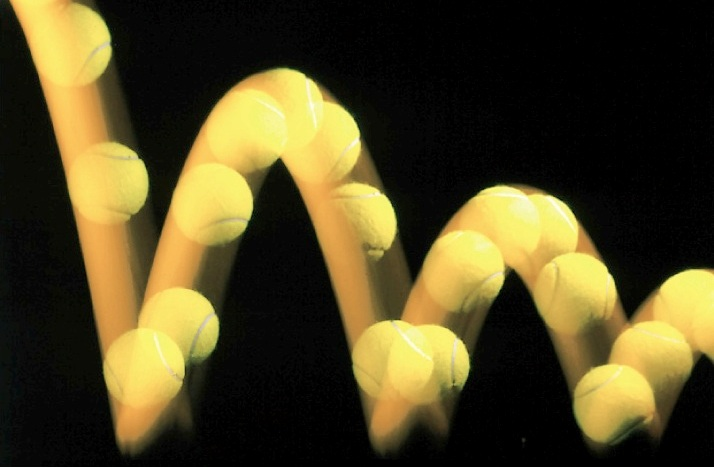
\includegraphics[width=0.8\textwidth]{stuiterendetennisbal}
\caption{Stuiterende tennisbal}\label{stuiterendetennisbal}
\end{figure}
Hoe lossen we dit probleem nu op? Als we naar de stroboscopische foto (\ref{stuiterendetennisbal}) van de stuiterende tennisbal kij\-ken, zien we dat de bal bovenaan trager beweegt dan wanneer hij de grond nadert. Bovenaan liggen de beelden immers dichter bij elkaar zodat de tennisbal minder afstand aflegt in de tijdsspanne tussen twee opeenvolgende opnames. 
De kwantitatieve\footnote{Kwantitatief wil zeggen dat het over een hoeveelheid of een grootte gaat.} informatie die we op deze manier uit de beelden kunnen destilleren, levert ons echter opnieuw gemiddelde snelheid en niet zomaar de ogenblikkelijke snelheid. De tennisbal verandert immers nog van snelheid tussen twee opeenvolgende opnames. Door nu echter de frequentie\footnote{Frequentie is een grootheid die aangeeft hoeveel cyclussen er per seconde worden doorlopen. Hier gaat het dus over het aantal beelden dat per seconde wordt gemaakt. De eenheid van frequentie is $\rm\,s^{-1}$ oftewel Hz (de Hertz).} waarmee de foto's worden genomen op te drijven, krijgen we een accurater beeld van de snelheid die de tennisbal op een gegeven moment heeft. De tijdsintervallen zijn nu immers korter zodat de bal minder van snelheid kan veranderen gedurende de intervallen en zodoende de gemiddelde snelheid een indicatie wordt van de ogenblikkelijke snelheid. De ogenblikkelijke snelheid wordt dus beter en beter benaderd door het tijdsinterval kleiner en kleiner en kleiner en kleiner\ldots te nemen. Echter, hoe kort het tijdsinterval ook is, de snelheid zal veranderen gedurende dat hele kleine tijdsinterval. Daarom, je raadde het misschien al lang, defini\"eren we de ogenblikkelijke snelheid als de \emph{limiet} van de gemiddelde snelheid over een tijdsinterval waarbij we dat interval naar nul laten gaan. Of m.a.w. wordt de ogenblikkelijke snelheid gedefinieerd \footnote{Dat betekent dus dat als iemand je vraagt wat snelheid is, je moet antwoorden dat het de afgeleide\ldots} als de afgeleide\footnote{De afgeleide is in deze context van het zoeken naar snelheid door Isaak Newton (1643-1727) en Gottfried Wilhelm von Leibniz (1646-1716) onafhankelijk van elkaar ontwikkeld.} van de plaatsfunctie:
\begin{eqnarray*}
v=\lim_{\Delta t\to 0}\frac{\Delta x}{\Delta t}=\lim_{t\to t_0}\frac{x(t)-x(t_0)}{t-t_0}=\frac{dx}{dt}
\end{eqnarray*}
We noteren dit ook zoals in de wiskunde met een accent $v(t)=x'(t)$ of $v=x'$. $v(t)$ is opnieuw een functie die op elk moment de snelheid geeft. 

Grafisch weet je dat je de afgeleide kan terugvinden als de richtingsco\"effici\"ent van de raaklijn. In een $x-t$ grafiek (de grafiek van de functie $x(t)$, $x$ in functie van $t$) vind je dus de snelheid als de richtingsco\"effici\"ent van een raaklijn in het beschouwde punt. 

Opmerking: Het woord 'ogenblikkelijk' mag je ook weglaten. Wanneer we het over snelheid hebben, bedoelen we vanaf nu steeds ogenblikkelijke snelheid.

\subsection{Ogenblikkelijke versnelling}

Voor een ogenblikkelijke verandering van de snelheid maken we eenzelfde redenering als voor de ogenblikkelijke verandering van de positie. De ogenblikkelijke versnelling wordt dus m.a.w. gewoonweg de afgeleide van de snelheid:
\begin{eqnarray*}
a=\lim_{t\to t_0}\frac{v(t)-v(t_0)}{t-t_0}&=&\frac{dv}{dt}=\frac{d^2x}{dt^2}
\end{eqnarray*}
Ook hier hanteren we eveneens een notatie m.b.v. accenten $a(t)=v'(t)=x''(t)$ en bedoelen we met versnelling, ogenblikkelijke versnelling.

\section{ERB}

De \emph{eenparig rechtlijnige beweging} (afgekort ERB) is een specifieke beweging. De snelheid van de beweging is eenparig of gelijkmatig verdeeld wat betekent dat de snelheid steeds gelijk blijft. M.a.w. is de snelheid constant of is de versnelling nul. Omdat de snelheid niet verandert is de ogenblikkelijke snelheid gelijk aan de gemiddelde snelheid en kunnen we gemakkelijk een functie vinden voor de positie in functie van de tijd:
\begin{eqnarray*}
v=\frac{\Delta x}{\Delta t}&\Leftrightarrow&\Delta x=v\Delta t\\
&\Leftrightarrow&x-x_0=v(t-t_0)\\
&\Leftrightarrow&x=x_0+v(t-t_0)
\end{eqnarray*}
Samengevat:

\kader{
%\vspace{3mm}
De plaatsfunctie $x(t)$ van een ERB met snelheid $v$ is gegeven door:
\begin{eqnarray}\label{x(t)ERB}
x(t)&=&x_0+v(t-t_0)
\end{eqnarray}
waarbij $x_0=x(t_0)$ de co\"ordinaat op het tijdstip $t_0$ is. Indien $t_0=0$ dan vereenvoudigt de plaatsfunctie (\ref{x(t)ERB}) tot
\begin{eqnarray}\label{x(t)ERB0}
x(t)&=&x_0+vt
\end{eqnarray}
%\vspace{0mm}
}

Aangezien de snelheid van een ERB constant is, is de beginsnelheid $v_0=v(t_0)$ gelijk aan de snelheid $v$, $v_0=v$. De snelheidsfunctie is natuurlijk $v(t)=v$ en de versnellingsfunctie is $a(t)=0$.
\begin{figure}[h]
\centering
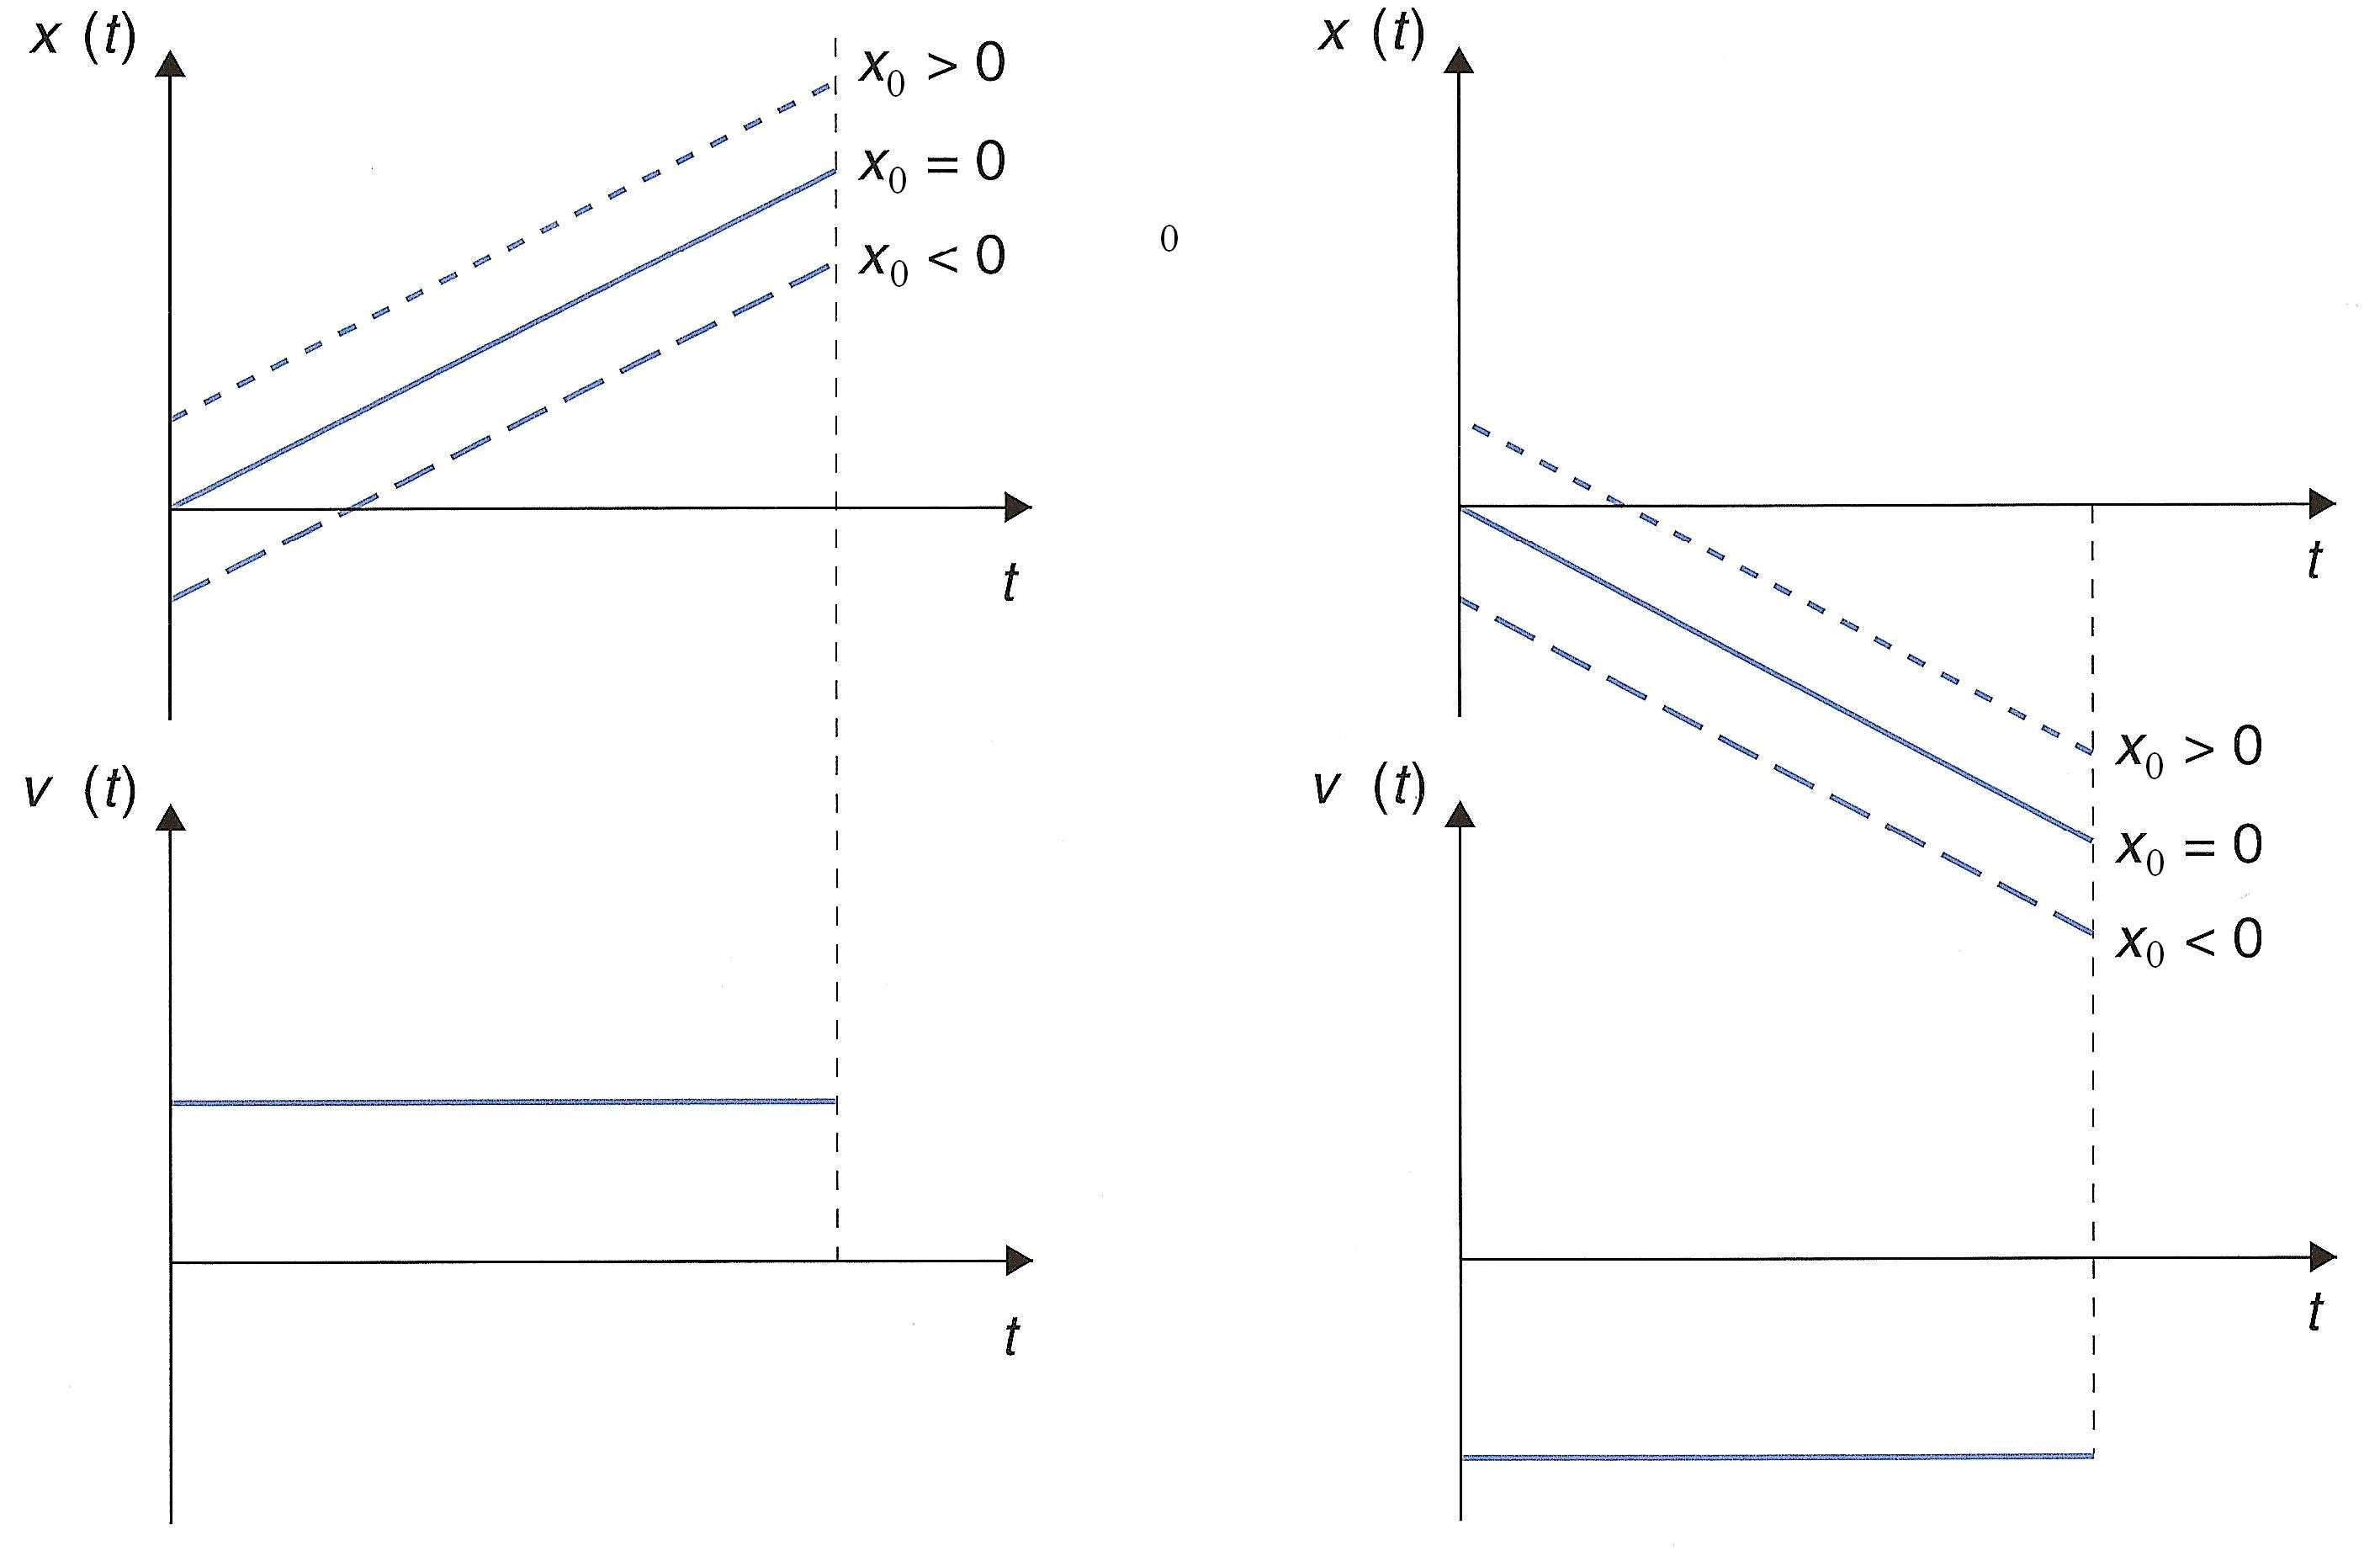
\includegraphics[width=.7\textwidth]{ERB_grafieken}
\caption{Grafieken van een ERB}
\end{figure}









\cleardoublepage
\setcounter{page}{1}
\setcounter{footnote}{0}
\setcounter{figure}{0}
\setcounter{equation}{0}
% 2021-2022: Aangepaste en verbeterde versie om als afzonderlijke bij lage aan de lln te kunnen geven.

\section{EVRB}

\section*{C Eenparig veranderlijke rechtlijnige beweging}

Een beweging waarvan de versnelling constant is, noemen we een \textit{eenparig veranderlijke rechtlijnige be\-we\-ging}, afgekort EVRB. Eenparig betekent gelijkmatig; de snelheidsverandering is steeds gelijk. In symbolen geldt dus dat $a(t)=a$ waarbij het maatgetal van $a$ een re\"eel getal is. We werken voor dit model de plaatsfunctie en de snelheidsfunctie uit. M.a.w. willen we het verloop van de plaats en de snelheid in functie van de tijd kennen. 

Aangezien de versnelling constant is en de versnelling de afgeleide van de snelheid, moet de snelheid in functie van de tijd een lineaire functie (in de tijd) zijn.\footnote{Strikt genomen zien we hier iets over het hoofd. A priori zou het immers kunnen dat er nog andere functies dan lineaire functies zijn waarvoor de afgeleide een constante functie is. Dat is echter niet het geval. Het bewijs hiervan zie je later dit jaar in het vak wiskunde. Je bewijst dat alle mogelijke functies die in aanmerking komen slechts op een constante na aan elkaar gelijk zijn.} Nu dat we het snelheidsverloop kennen, kunnen we het verloop van de plaats afleiden. Aangezien de snelheid een lineaire functie is en de snelheid de afgeleide van de positie is, moet de positie een kwadratische functie (in de tijd) zijn. De afgeleide van een kwadratische functie is immers een lineaire functie.\footnote{Hier geldt een gelijkaardige opmerking als die in de vorige voetnoot.}

Dat de positie in functie van de tijd een tweedegraadsveeltermfunctie is, geeft in symbolen:\footnote{we gebruiken de constanten $p$, $q$ en $r$ i.p.v. $a$, $b$ en $c$ om verwarring met de betekenis van $a$ te voorkomen.}
\begin{eqnarray}
x(t)=pt^2+qt+r\label{pqr}
\end{eqnarray}
Nu willen we de constanten $p$, $q$ en $r$ fysisch kunnen duiden en eventueel andere symbolen geven, zodat hun betekenis sneller af te lezen is. Dat doen we door te eisen dat de afgeleide met de snelheid overeenkomt en de tweede afgeleide met de versnelling. Ook gebruiken we de beginvoorwaarden. Dus:
\begin{align}
v(t)&=\frac{dx}{dt}=2pt+q\label{2pq}\\
a(t)&=\frac{d^2x}{dt^2}=2p\nonumber
\end{align}
Omdat de versnelling constant is, halen we uit de laatste regel dat $a(t)=a=2p\Leftrightarrow p=\frac{a}{2}$. Als we met $v_0$ de snelheid op tijdstip $t=0$ voorstellen ($v_0=v(0)$) en $t=0$ invullen in (\ref{2pq}), dan vinden we dat $q=v_0$. De constante $q$ stelt dus de beginsnelheid voor. Als we vervolgens met $x_0$ de positie op tijdstip $t=0$ voorstellen en $t=0$ invullen in (\ref{pqr}), dan vinden we dat $r=x_0$. De constante $r$ stelt dus de beginpositie voor.

Samengevat levert dat:

\kader{
%\phantom{}
\vspace{1ex}
De plaatsfunctie $x(t)$ en de snelheidsfunctie $v(t)$ van een EVRB met versnelling $a$ worden gegeven door:
\begin{eqnarray}
x(t)&=&x_0+v_0t+\frac{1}{2}at^2\label{x(t)0}\\
v(t)&=&v_0+at\label{v(t)0}
\end{eqnarray}
Hierin is $x_0$ de \textit{beginpositie} en $v_0$ de \textit{beginsnelheid}. Ze worden bepaald door de \textit{beginvoorwaarden} of \textit{randvoorwaarden}.
\vspace{1ex}
%\phantom{.}
}

Indien we de beschrijving van de beweging niet op $t=0$ willen laten starten maar op een gegeven tijdstip $t_0$, dan moeten we in de beschrijving $t$ vervangen door $\Delta t= t-t_0$, de verstreken tijd vanaf het begintijdstip $t_0$. De functies (\ref{x(t)0}) en (\ref{v(t)0}) worden dan een klein beetje ingewikkelder:
\begin{eqnarray}
x(t)&=&x_0+v_0(t-t_0)+\frac{1}{2}a(t-t_0)^2\label{x(t)}\\
v(t)&=&v_0+a(t-t_0)\label{v(t)}
\end{eqnarray}

Met de functies (\ref{x(t)}) en (\ref{v(t)}) kunnen we de volgende formule voor de gemiddelde snelheid van een EVRB aantonen:%\footnote{Het formuletje is handig te gebruiken in veel vraagstukken door gebruik te maken van $\Delta x=\overline{v}\Delta t$.} 
\footnote{De afleiding van de gemiddelde snelheid is als volgt:
\begin{eqnarray*}
\overline{v}=\frac{\Delta x}{\Delta t}=\frac{x-x_0}{t-t_0}=\frac{v_0(t-t_0)+\frac{1}{2}a(t-t_0)^2}{(t-t_0)}=\frac{2v_0+a(t-t_0)}{2}=\frac{v_0+v}{2}.
\end{eqnarray*}}
\begin{eqnarray*}
  \overline{v}=\frac{v_0+v}{2}
\end{eqnarray*}
Blijkbaar houdt het eenparig toenemen van de snelheid in dat we het rekenkundig gemiddelde kunnen gebruiken voor de gemiddelde snelheid.

\newpage

\begin{figure}[h]
\centering
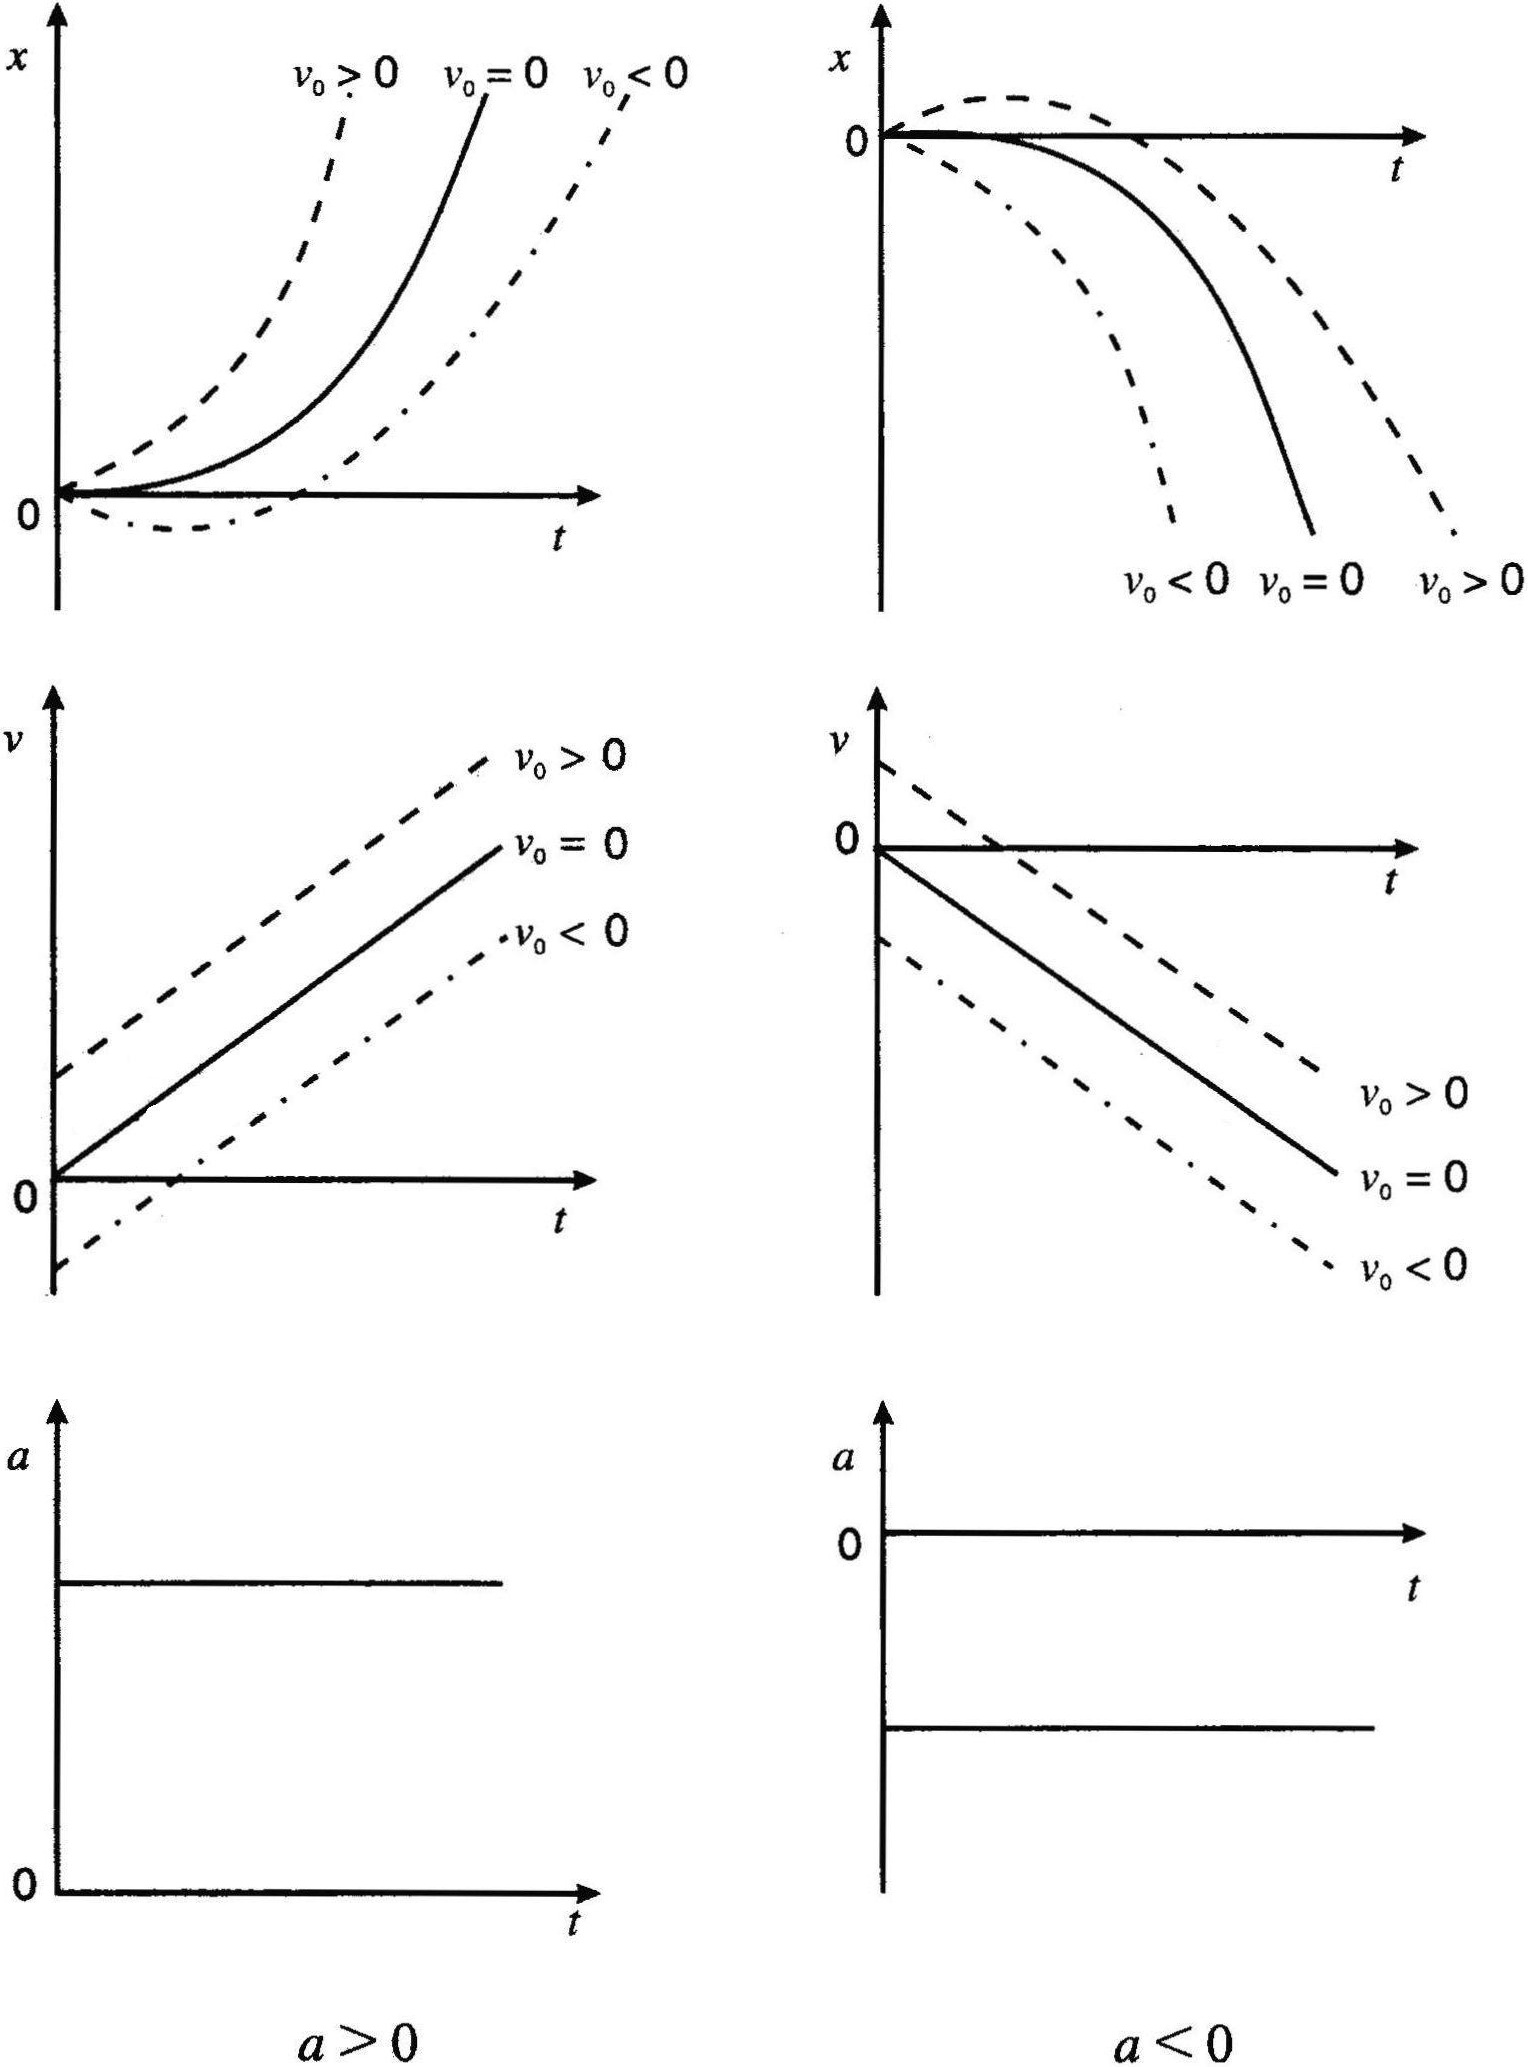
\includegraphics[width=\textwidth]{EVRB_grafieken}
%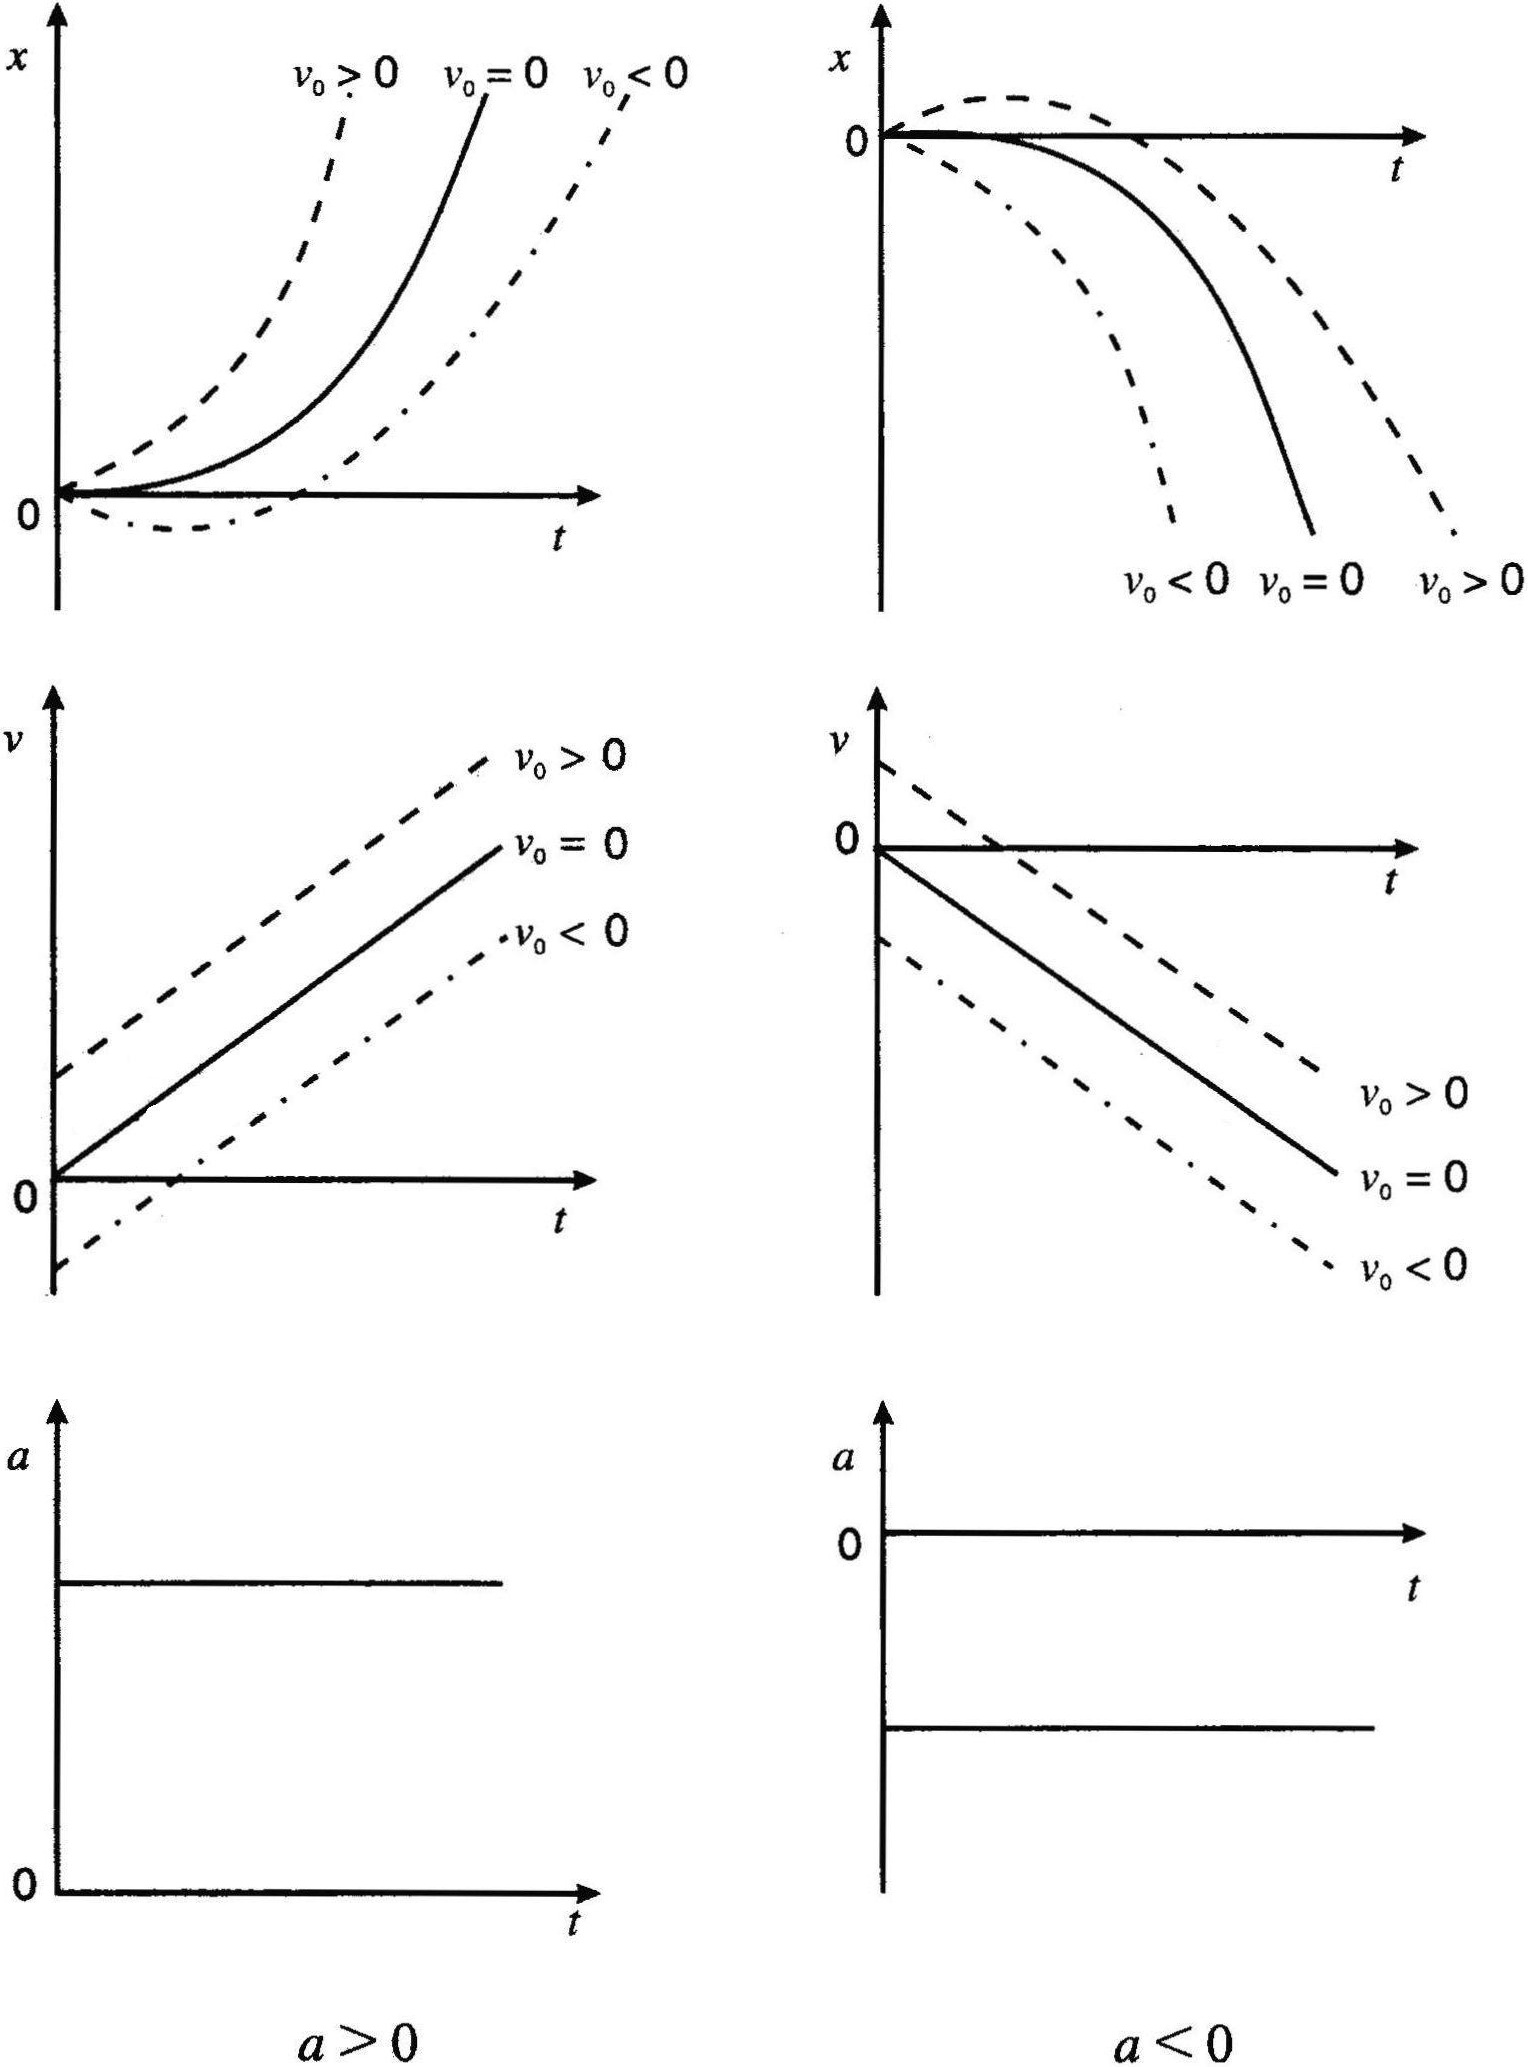
\includegraphics[height=\textheight]{EVRB_grafieken}
\caption{Grafieken van een EVRB}
\end{figure}

\clearpage
\newpage
\thispagestyle{empty}

\section*{Voorbeeldoefening}

\begin{enumerate}

\item[\textbf{Opgave}]\textsf{Een auto die $\SI{60}{km/h}$ rijdt, raakt een boom; de voorkant van de auto wordt in elkaar gedrukt en de bestuurder komt na $\SI{70}{cm}$ tot stilstand. Welke gemiddelde vertraging onderging de bestuurder tijdens de botsing? Druk je antwoord uit in $g$, waarbij $g=\SI{9,81}{m/s^2}$.
\item[\textit{Gegeven}]$v_0=\SI{16,7}{m/s}$\newline$x=\SI{0,70}{m}$
\item[\textit{Gevraagd}]$a$
\item[\textit{Oplossing}] Om de (constante) vertraging te vinden, hebben we de snelheidsverandering en de benodigde tijd nodig. De verandering in snelheid kennen we; de eindsnelheid van de auto moet nul worden maar de duur is niet onmiddellijk gegeven. Omdat de eindsnelheid nul is, kunnen we wel uit de snelheidsvergelijking van een eenparig veranderlijke beweging een \emph{uitdrukking} vinden voor die tijd die we vervolgens kunnen substitueren in de plaatsvergelijking. De enige onbekende is dan de gezochte versnelling.\footnote{M.b.v. de formule $\overline{v}=\frac{v_0+v}{2}$ voor de gemiddelde snelheid en de definitie voor de gemiddelde snelheid $\overline{v}=\frac{\Delta x}{\Delta t}$ is het antwoord sneller te vinden. Ga maar na \ldots}
\newline
\newline
Uit $v(t)=0$ of $0=v_0+at$ halen we een uitdrukking voor de tijd die nodig is om tot stilstand te komen:
\begin{align*}
t&=-\frac{v_0}{a}
\end{align*}
Substitutie van deze tijd in de plaatsfunctie levert:
\begin{align*}
x&=v_0t+\frac{1}{2}at^2\\
&=v_0\left(-\frac{v_0}{a}\right)+\frac{1}{2}a\left(-\frac{v_0}{a}\right)^2\\
%&=&-\frac{v_0^2}{a}+\frac{v_0^2}{2a}\\
&=-\frac{v_0^2}{2a}\\
\end{align*}
De versnelling is dan gelijk aan:
\begin{align*}
a&=-\frac{v_0^2}{2x}
\end{align*}
Invullen van de gegevens levert $a=\SI{-198}{m/s^2}$, wat gelijk is aan $20g$.
}
\end{enumerate}

\newpage










\section{Verticale worp}

Onze perceptie van vallende voorwerpen is dat zwaardere lichamen sneller vallen dan lichtere. Een veertje en een hamer komen in de regel niet tegelij\-ker\-tijd op de grond terecht. Wanneer we echter voorwerpen in vacu\"um\footnote{In vacu\"um ondervinden voorwerpen geen luchtweerstand.} laten vallen, blijkt de massa geen rol te spelen bij de constante versnelling die de voorwerpen krijgen -- alle voorwerpen vallen met dezelfde versnelling. De verklaring hiervoor hoort thuis in de dynamica. In de kinematica houden we ons enkel bezig met de beschrijving van de beweging. Aangezien de valversnelling constant is, hebben we simpelweg met een EVRB te maken.
\begin{figure}[h]
\centering
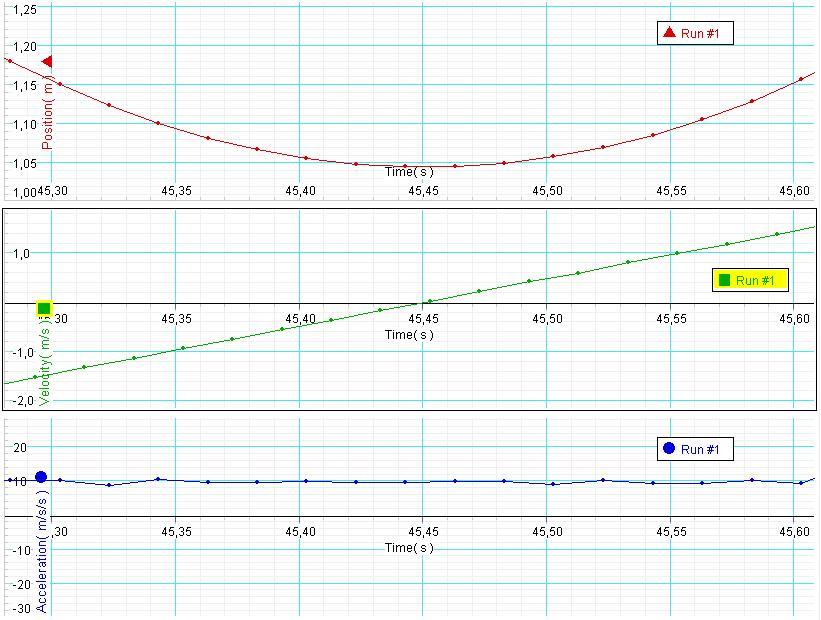
\includegraphics[width=0.85\textwidth]{valbeweging_pasco2}
\caption{Experimenteel bekomen grafieken van een verticale worp waarbij de as naar beneden is geori\"enteerd.}
\end{figure}
Strikt genomen verschilt de valversnelling van plaats tot plaats op de aarde, maar voor het gemak nemen wij in vraagstukken de waarde
\[g=9,81\rm\,m/s^2.\]
Omdat de verticale worp een EVRB is, kunnen we de formules (\ref{x(t)0}) en (\ref{v(t)0}) gebruiken om een valbeweging te beschrijven. Voor de versnelling $a$ nemen we dan $a=g$ of $a=-g$ al naargelang de ori\"entatie van de co\"ordinaatas.

\clearpage
\newpage


\begin{enumerate}
\item[\textbf{Opgave}]\textsf{Van de boord van een schip valt een loden bol in het water. De \mbox{boord} bevindt zich $4,0\rm\,m$ boven het wateroppervlak. De loden bol zinkt vervolgens met de snelheid waarmee hij het water raakte. Er zijn $6,0\rm\,s$ tussen het tijdstip waarop de bol valt en ze de bodem van het water bereikt.
\begin{enumerate}
\item Hoe diep is het water?
\item Wat is de gemiddelde snelheid van de bol over het hele traject?
\end{enumerate}
\item[\textit{gegeven}]$x_1=4,0\rm\,m$\newline$t_2=6,0\rm\,s$
\item[\textit{gevraagd}]$x_2-x_1$, $\overline{v}_{02}$
\item[\textit{oplossing}]De beweging is opgebouwd uit twee verschillende soorten bewegingen. Het eerste stuk is een vrije val, wat een EVRB is. In het tweede stuk (onder water) is de snelheid constant en is er dus geen versnelling. In geen geval kunnen we dus de formules voor een EVRB op het geheel toepassen. Die zijn immers afgeleid voor een beweging waar de versnelling (altijd, gedurende de hele beweging) constant is.
\begin{figure}[h]
\centering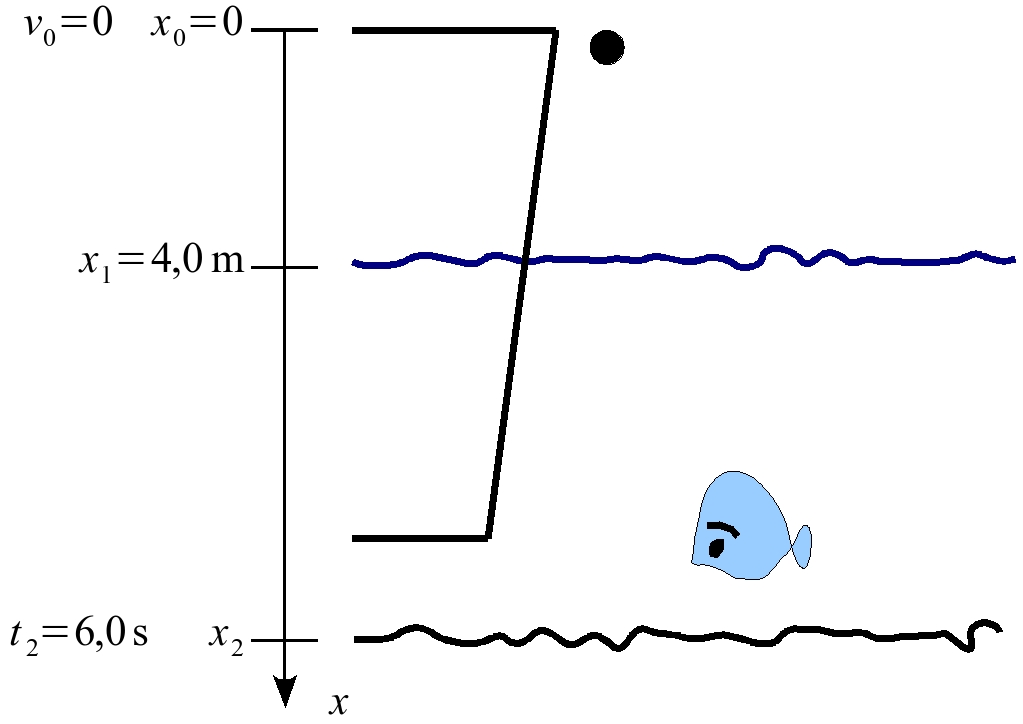
\includegraphics[width=0.4\textwidth]{boordschip}
\end{figure}
Omdat we weten hoe ver de bol moet vallen voordat hij het wateroppervlak bereikt, kunnen we zowel de tijd die de bol hiervoor nodig heeft als de snelheid waarmee de bol het wateroppervlak raakt, bepalen. We kiezen een as naar beneden zodat -- omdat de snelheid in deze richting toeneemt -- de versnelling positief is en gelijk aan de valversnelling $g$ (toch voor het eerste stuk). De beginsnelheid van de bol is nul omdat hij vanuit rust wordt losgelaten. Voor de tijd vinden we:
\begin{eqnarray}
x_1=\frac{1}{2}gt^2\quad\Rightarrow\quad t_1&=&\sqrt{\frac{2x_1}{g}}\label{tijd_boordschip}
\end{eqnarray}
Met de tijd\footnote{We zouden de tijd met het gevonden formuletje kunnen uitrekenen en met het getalletje dat we vinden verder rekenen. Maar met het formuletje verder werken -- algebra\"isch of symbolisch -- is toch o zo veel knapper en van toepassing voor \'alle boten en niet enkel voor een boot waarvoor het dek zich $4,0$ meter boven het wateroppervlak bevindt. Bovendien is het ``echte'' fysica omdat je een ``model'' uitwerkt en niet een rekensommetje oplost...} kunnen we de snelheid op het wateroppervlak vinden.
\begin{eqnarray}
v_1=gt_1\nonumber=g\sqrt{\frac{2x_1}{g}}\nonumber=\sqrt{2gx_1}\label{snelheid_boordschip}
\end{eqnarray}
Onder water, in het tweede stuk, beweegt de kogel met deze snelheid gedurende de resterende tijd: $6,0$ seconden min de tijd $t_1$ (\ref{tijd_boordschip}) die de kogel nodig had om te vallen. De afstand die de bol onder water aflegt, vinden we met de eenvoudige formuletjes van een ERB\footnote{Opmerking, een ERB is een speciaal geval van een EVRB. Een ERB heeft als constante versnelling $a=0$.}. We substitueren ook vergelijkingen (\ref{tijd_boordschip}) en (\ref{snelheid_boordschip}).
\begin{eqnarray*}
\Delta x&=&\overline{v}\cdot\Delta t\\
&\Downarrow&\\
x_2-x_1&=&v_1(t_2-t_1)\\
&=&\sqrt{2gx_1}(t_2-\sqrt{\frac{2x_1}{g}})\\
&=&\sqrt{2gx_1}t_2-2x_1\\
&=&45\rm\,m
\end{eqnarray*}
De gemiddelde snelheid vinden we door de totale afgelegde weg te delen door de totale benodigde tijd. Andere formuletjes zoals $\overline{v}=\frac{v_1+v_2}{2}$ zijn niet van toepassing omdat het helemaal niet over \'e\'en EVRB gaat waar dit formuletje geldt omdat de snelheid mooi lineair toeneemt. Hier gebeurt dat enkel in het eerste stuk en worden de verschillende snelheden niet even lang aangehouden zodat ze een verschillend aandeel hebben in de totale benodigde tijd.
\begin{eqnarray*}
\overline{v}_{02}=\frac{\Delta x}{\Delta t}=\frac{x_2}{t_2}&=&\frac{\sqrt{2gx_1}t_2-x_1}{t_2}\\
&=&\sqrt{2gx_1}-\frac{x_1}{t_2}\\
&=&8,2\rm\,m/s
\end{eqnarray*}}
\end{enumerate}

\cleardoublepage
\newpage